% !TEX root = main.tex

\section{はじめに}

\section{関連研究}
\label{sec:relatedwork}

\subsection{\Bctree{}}
\subsection{Masstree}

\section{\Bcforest{}の構造}
\label{sec:bc_forest_structure}

\section{\Bcforest{}のノード操作}
\label{sec:node_operation}
本節では,\Bcforest{}のノード操作について述べる.
\Bcforest{}は以下の読み取りおよび書き込み操作をサポートする.

\subsection{書き込み}
% 書き込み操作の概要
書き込み(Write)はキーとペイロードを差分レコード領域に挿入する操作である.
まず,キーの先頭0~7~byteが属するの葉ノードを根ノードから二分探索により特定する(Layer0).
次に,葉ノード内のイミュータブル領域を二分探索し,接頭辞8~byteが共通するキーについて下層へのポインタの有無を確認する.
ポインタが無い場合,本葉ノードを挿入先の葉ノードとして特定する.
ポインタがある場合,下層の根ノードへ移動し,キーの8~15~byteが属する葉ノードを二分探索により特定する(Layer1).
本操作を下層ポインタがなくなるまで繰り返し,葉ノードを特定する.
挿入先の葉ノードに到達後,その葉ノードの差分レコード領域に値を挿入する.

% 書き込み操作の具体的な手順
書き込み操作は差分レコード領域の予約とレコード挿入および可視化の2ステップで行われる.
\Fig{\ref{fig:bc_tree_insertion}}に\Bctree{}における差分レコードの挿入を示す.
ノードフッタにはミュータブル領域の状態を表すステータスワードを用意し,この中のレコード数と使用済みブロックサイズを加算することで差分レコード用の領域を予約する.
また,\Bctree{}ではノードの生成時にミュータブル領域をゼロ埋めしている.
\Bctree{}では,メタデータがゼロ埋めされている場合を処理途中として表すため,差分レコード用の領域を予約した時点ではレコードが可視化されていないことを認識できる.
確保した領域へ差分レコードを書き込み,対応するレコードメタデータの値を更新することでレコードを可視化し,挿入処理を完了する.

\begin{figure}[t]
    \centering
    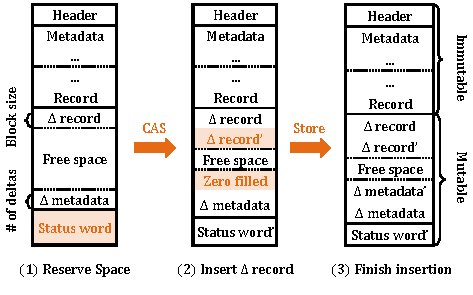
\includegraphics{./figures/Bc-insertion.pdf}
    \caption{\Bctree{}における差分レコードの挿入}
    \label{fig:bc_tree_insertion}
\end{figure}

% 書き込みができない場合の対処
以上の書き込み操作によって差分レコードを挿入していくが,挿入後の差分レコードの総数またはノード容量のしきい値を越える場合,差分レコードの統合操作または構造変更操作が行われる.
しきい値の確認はステータスワードの更新時に行われ,しきい値を越えた場合はレコードの書き込み後に統合操作,構造変更操作いずれかの操作を行うか判定する.

% Bc木の書き込み操作の特徴
書き込み処理はロックフリーに動作する.
書き込み同士の競合はステータスワードで解決され,差分レコード用領域の予約,つまり差分レコードの書き込み順はCAS命令の成功順によって順序付けられる.
また,後述する構造変更操作との競合によって待ち時間が発生しうる.

\subsection{読み取り}
% 読み取り操作の概要とミュータブル領域での読み取り
読み取り(Read)は与えられた対象キーのペイロードを返す操作である.
まず,キーの先頭0~7~byteが属するの葉ノードを根ノードから二分探索により特定する(Layer0).
葉ノードに到達した後は,葉ノード内の差分レコードの線形探索とイミュータブルレコードの二分探索の2ステップで読み取り操作を行う.
最新の値は差分レコード領域に書き込まれるため,まずミュータブル領域を線形探索し,一致するキーがあるか確認する.
このとき,差分レコードの数はステータスワードから読み取り,差分レコードが可視化されていなければスキップする.

% ミュータブル領域にレコードがない場合
差分レコード中に対象のレコードが存在しなければ,ノードヘッダからイミュータブルレコードの数を読み取り,二分探索によって対象キーの有無を確認する.
接頭辞8~byteが共通するキーについてposting listが存在する場合には,posting list内を線形探索し,接尾辞が一致するキーがあるか確認する.
接頭辞8~byteが共通するキーについて下層へのポインタが存在する場合には,下層の根ノードへ移動する(Layer0→Layer1).
Layer1移動後,キーの8~15~byteが属する葉ノードを二分探索により特定し,同様の2ステップを行う(Layer1).
この操作を下層へのポインタがなくなるまで繰り返し,読み取り操作を行う.
先頭ノードが統合操作の途中である場合には,差分レコードを読み終わった時点で物理ポインタをたどり古いノードへ移動し,同様の2ステップを古いノード上で行う.

% Bc木における読み取り操作の特徴
読み取り処理はwait-freeに動作する.
上述したとおり読み取り命令は一切ノードの状態を変更せず,読み取った状態に応じて適切な手続きを選択する.
そのため,読み取り命令においてリトライなどは発生せず,有限時間内で必ず処理が終了する.

\section{\Bcforest{}の構造変更操作}
\label{sec:smo}

\subsection{統合}
\subsection{分割}
\subsection{新層作成}

\section{おわりに}
\label{sec:conclusion}

